% TEX STUDIO MAGIC-COMMAND
% !TeX document-id = {21ffa6e2-6c8f-4532-897c-386dc477f19a}
% !TeX root = abstract.tex
% !TeX encoding = utf8
% !TeX TXS-program:compile = lualatex -file-line-error -synctex=1 -interaction=nonstopmode -halt-on-error %.tex
% !TeX TXS-program:quick = txs:///compile | txs:///view-pdf-internal --embedded
%%% TeXのファイル名を変えたら ↑ も変えましょう



%%%-------------------------------------------------------------------------
%%% PD3予稿集テンプレート (main.tex)
%%% 作成: 金沢工大・情報工学科・鷹合研究室(2022,01/12)
%%%-------------------------------------------------------------------------

%%%%%%%%%%%%%%%%%%%%%%%%%%%%%%%%%%%%%%%%%%%%%%%%%%%%%%%%%%%%%%%%%%%%%%%%%%%
%                               テーマ,著者情報をここに書き込んでください
%ここから ------------------------------------------------------------------

%%% テーマ番号x
\def\THEMEID{1EP001}

%%% タイトル
\def\TITLEJP{機械学習を用いた電車の車両タイプ判別システムの開発}
\def\TITLEEN{Development of a Train Type Identification System Using Machine Learning}
\def\CENTERADJ{3.3} % ここを書き換えて,表紙の「プロジェクトテーマ」という文字列がセル中心になるよう調整してください

%%% 教員名
\def\PROFNAME{鷹合 大輔 准教授}

%%% アブストラクト(英文で書く)
% 最低:100ワード,最大:300ワード前後
% 英文部分については,句読点は半角にすること.つまり", "か". "を使う
\def\ABSTRACT{
	There are nearly 100 types of train cars for JR’s conventional lines alone. There are nearly 100 types of train cars on JR’s
	conventional lines alone. It is difficult for those who do not have much knowledge of trains to distinguish similar train car types. In this
	project This project aims to create a system to identify train car types using YOLO. The classification and discrimination models were
	created using the same image dataset, and the discrimination results were similar. A web application was also created using the created
	model.Created a web application and server using nodejs to output discrimination results .
%There are nearly 100 types of train cars for JR's conventional lines alone.
%There are nearly 100 types of train cars on JR's conventional lines alone. It is difficult for those who do not have much knowledge of trains to distinguish similar train car types. In this project
%This project aims to create a system to identify train car types using YOLO. The classification and discrimination models were created using the same image dataset, and the discrimination results were similar. A web application was also created using the created models.
%Describe about 5 lines of abstract in English here. Describe about 5 lines of abstract in English here. Describe about 5 lines of abstract in English here. Describe about 5 lines of abstract in English here. Describe about 5 lines of abstract in English here. Describe about 5 lines of abstract in English here. 
%\textbf{(何が問題で,それをどんな手法で取り組んで,どういう結果であったかなどを英語で要約して下さい)}
 %Describe about 5 lines of abstract in English here. Describe about 5 lines of abstract in English here. Describe about 5 lines of abstract in English here.
}

%%% キーワード(5個まで)
\def\KEYWORDS{YOLO,Machine Learning,node.js,python-shell,python}

%%% 著者リスト
\def\AUTHORS{
\begin{minipage}{13.5cm}
~\hfill 4EP1-68~野崎 悠渡(NOZAKI Yuto)      ~~~~~ 4EP4-75~田村 優祐(TAMURA Yusuke) \hfill~
\end{minipage}
}

\newcommand{\red}[1]{\textcolor{red}{#1}}


% テーマ,著者情報ここまで -----------------------------------------------------


%%%%%%%%%%%%%%%%%%%%%%%%%%%%%%%%%%%%%%%%%%%%%%%%%%%%%%%%%%%%%%%%%%%%%%%%%%%%
%                                本文


\documentclass{tkglabs}

\usepackage{caption}

\begin{document}
\maketitle
\begin{multicols*}{2} % *アスタ付きだとページのバランシングを無効にできる
%本文ここから ------------------------------------------------------------------



\section{はじめに}
%背景や目的をここに書いてください.
電車の車両タイプはJRの在来線だけでも100種類近く存在している.
電車の知識がある人は一目見るだけでその電車の車両タイプを判別できるが,電車の知識があまりない人は似ている電車の車両タイプを判別することが難しい.本プロジェクトでは簡単に画像や動画に写っている車両タイプが何なのかを分類または識別できるシステムを開発する.

\section{画像の分類と識別について}
画像の分類とは,画像が特定のカテゴリやクラスに属するかどうかを判別する作業である.例えば,画像に写っているのが猫か犬かのクラスに分けることである.

識別とは画像のどこに何が写っているのかを判別するプロセスを指す.1枚の画像に複数の物体が存在する場合も識別はできる.動画に写っている電車の車両タイプも判別することができる.
%\section{関連研究?現存するサービスについて?これいる??}
%先行事例と本システムの独自性
%googleがgoogleレンズというサービスを提供している.これは,画像に写っている物体と同じものが写っているウェブサイトをまとめて表示するサービスである.このサービスの問題点は3つある.
%\begin{itemize}
%	\item 一枚の画像に複数の物体が写り込んでいると判別結果が正確ではなくなる.
%	\item 提示されたウェブサイトから詳細を確認しなければならない.
%	\item 動画から物体を判別することができないこと
%\end{itemize}

\section{システム概要}
%開発するシステムの概要を図 \ref{abc}に示す.
本システムは,ユーザに画像または動画をブラウザ上で入力してもらい,それをサーバ上で画像認識を用いて処理し,結果をブラウザで表示するWebアプリケーションである.Webサイトのテンプレートにはw3.school~\cite{bk0}のものを使用した.システム概要を図\ref{abc}に示す.
\begin{figure} % 小さな図
	\label{abc}
	\centering
	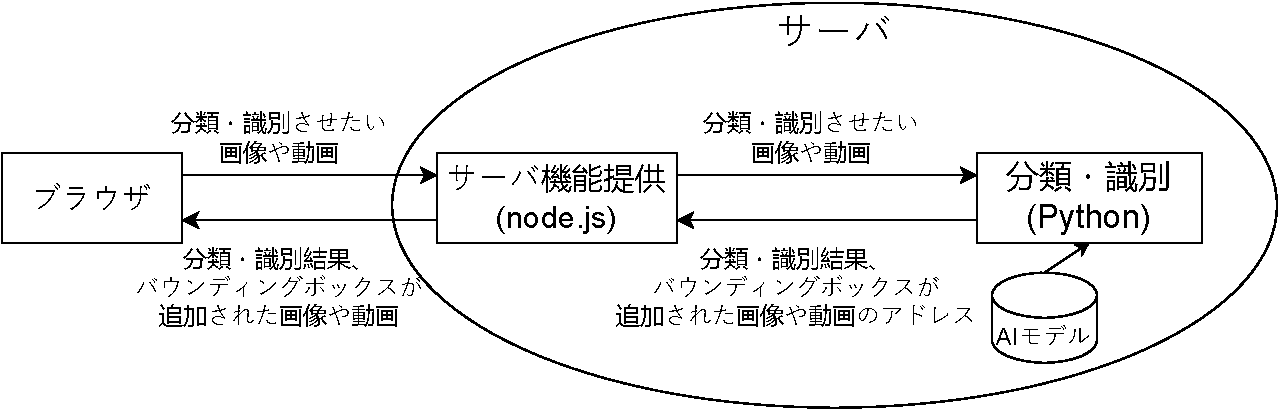
\includegraphics[width=\linewidth]{obj/sys_gaiyou6.pdf}
	\figcap{システム概要}{System Overview}{abc}
\end{figure}

\section{システムの機能}
%本システムの機能として電車の分類と識別を提供する.識別は動画と画像の両方に対応している.
%画像や動画を入力すると,判別結果が出力される.
本システムは,以下の3つの機能を提供する.
%本システムは,電車の画像の分類と電車の画像と動画の識別の3つ機能を提供する
\begin{itemize}
	\item 電車の画像の分類
	\item 電車の画像の識別
	\item 電車の動画の識別
\end{itemize}


\subsection{電車の画像の分類} 
出力後の画面を図\ref{img_cls}に示す.
この機能では,ユーザがブラウザからアップロードした画像に含まれる電車の種類を分類する. 分類の結果,最も可能性が高いものをWebページに出力する.
\subsection{電車の画像の識別}
出力後の画面を図\ref{img_det}に示す.
この機能では,ユーザがブラウザからアップロードした画像に含まれる電車の位置と種類を識別する.  識別の結果,バウンディングボックスが追加された画像をWebページに表示する.
\subsection{電車の動画の識別} 
出力後の画面を図\ref{mov_det}に示す.
この機能では,ユーザがブラウザからアップロードした動画に含まれる電車の位置と種類を識別する. 識別の結果,バウンディングボックスが追加された動画をWebページに表示する.

%\begin{figure}
%	\centering
%	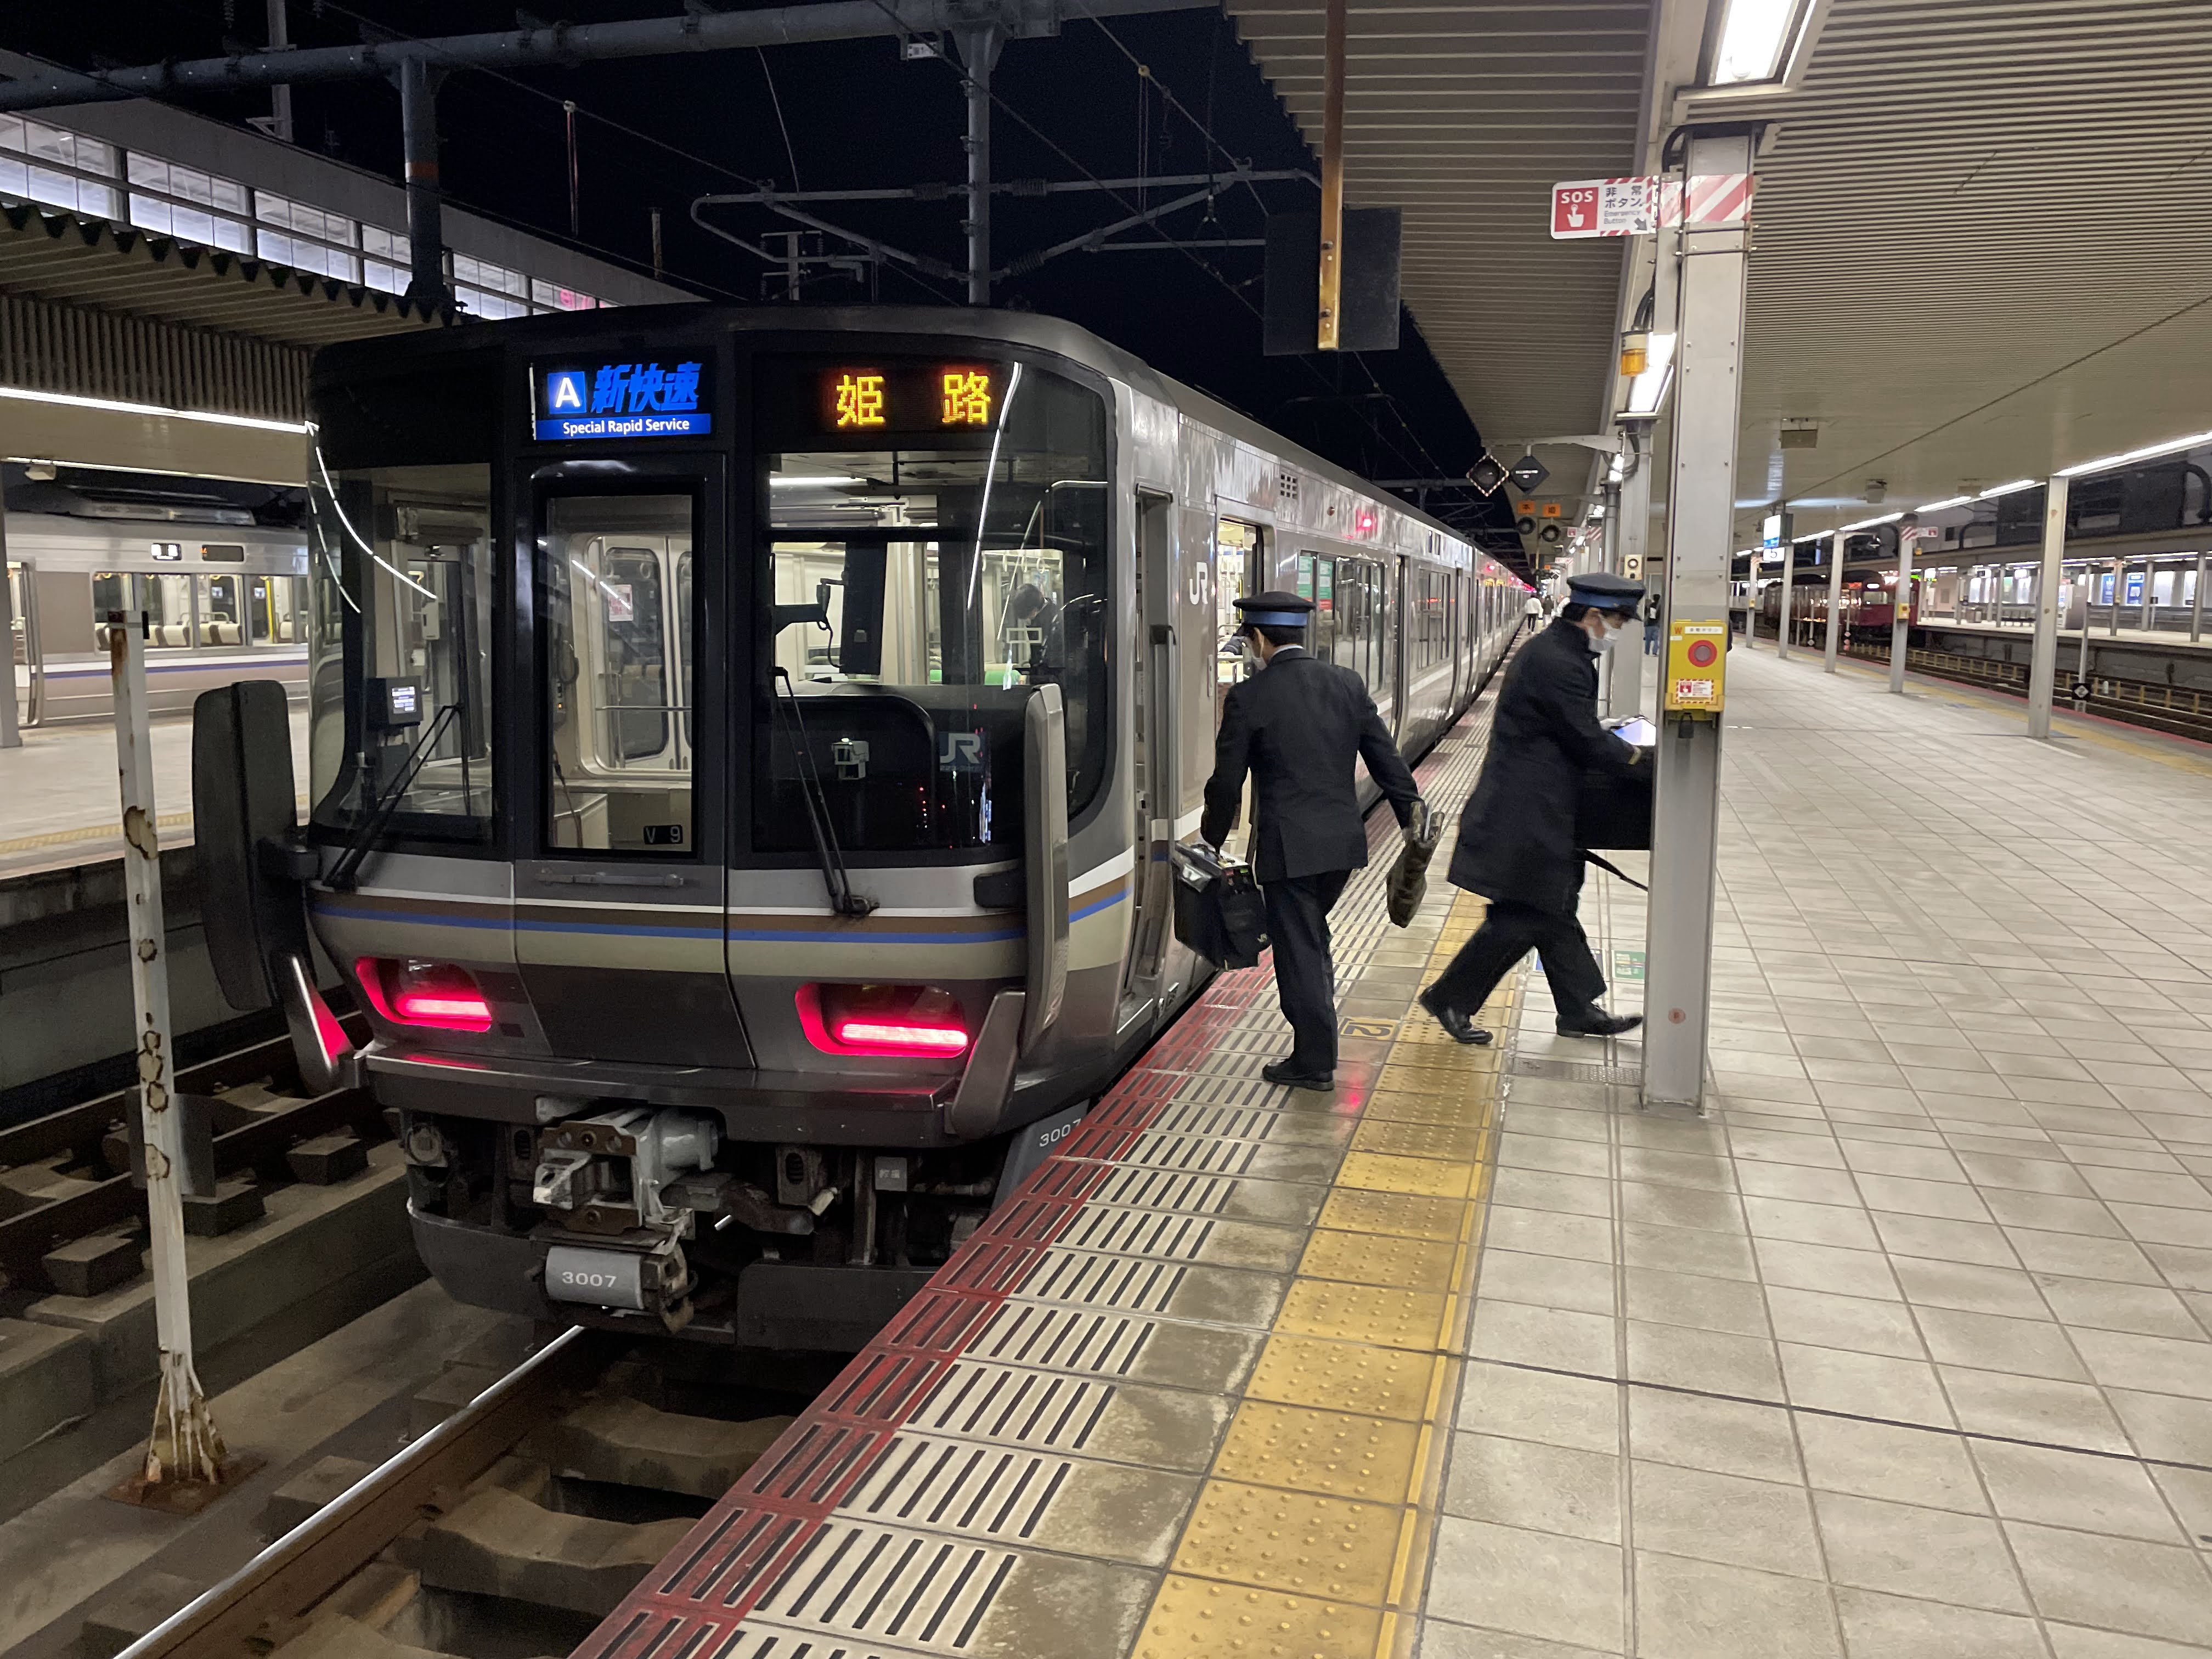
\includegraphics[width=0.5\linewidth]{obj/image1.png}
%	\figcap{画像の分類}{classify image}{cls-img}
%\end{figure}

\begin{figure}
	\begin{tabular}{ccc}
		\begin{minipage}[b]{0.3\textwidth}
			\centering
			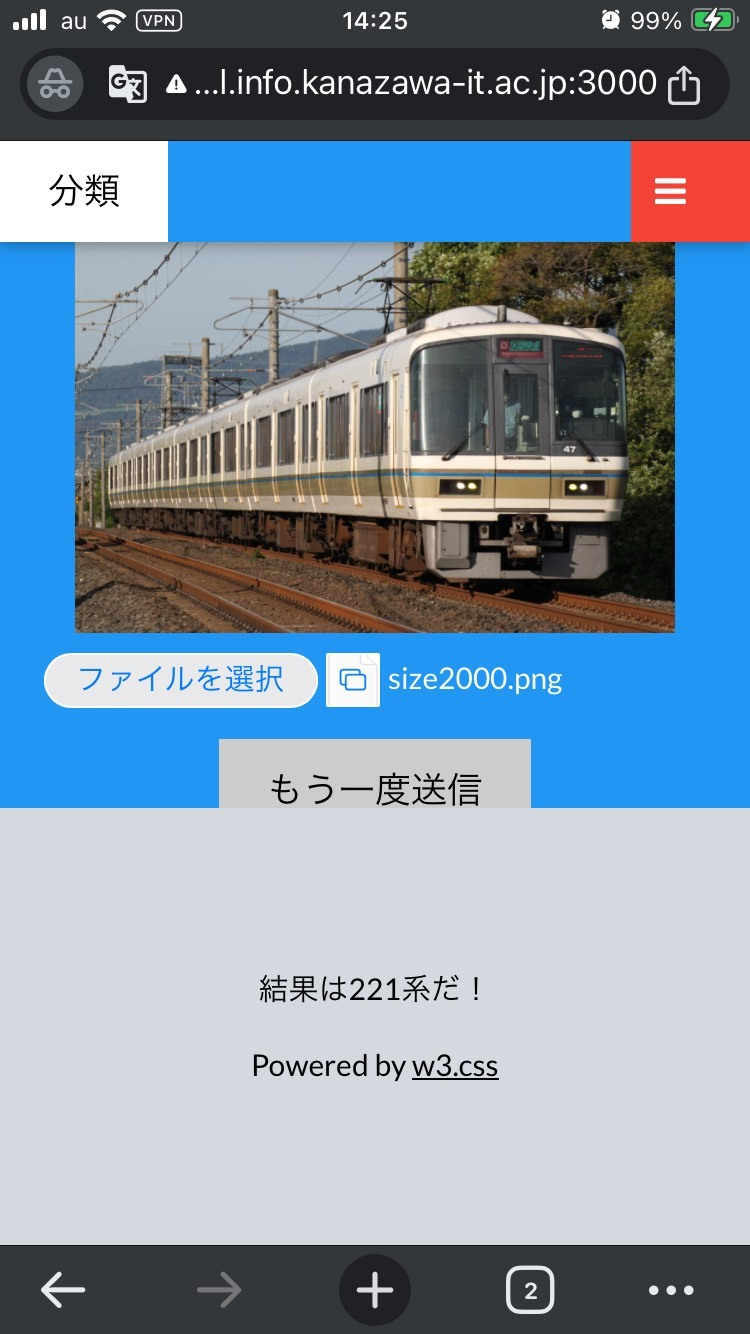
\includegraphics[width=\linewidth]{obj/img_classify.jpg}
			\figcap{画像の分類}{Image Classification}{img_cls}
		\end{minipage}
		\begin{minipage}[b]{0.3\textwidth}
			\centering
			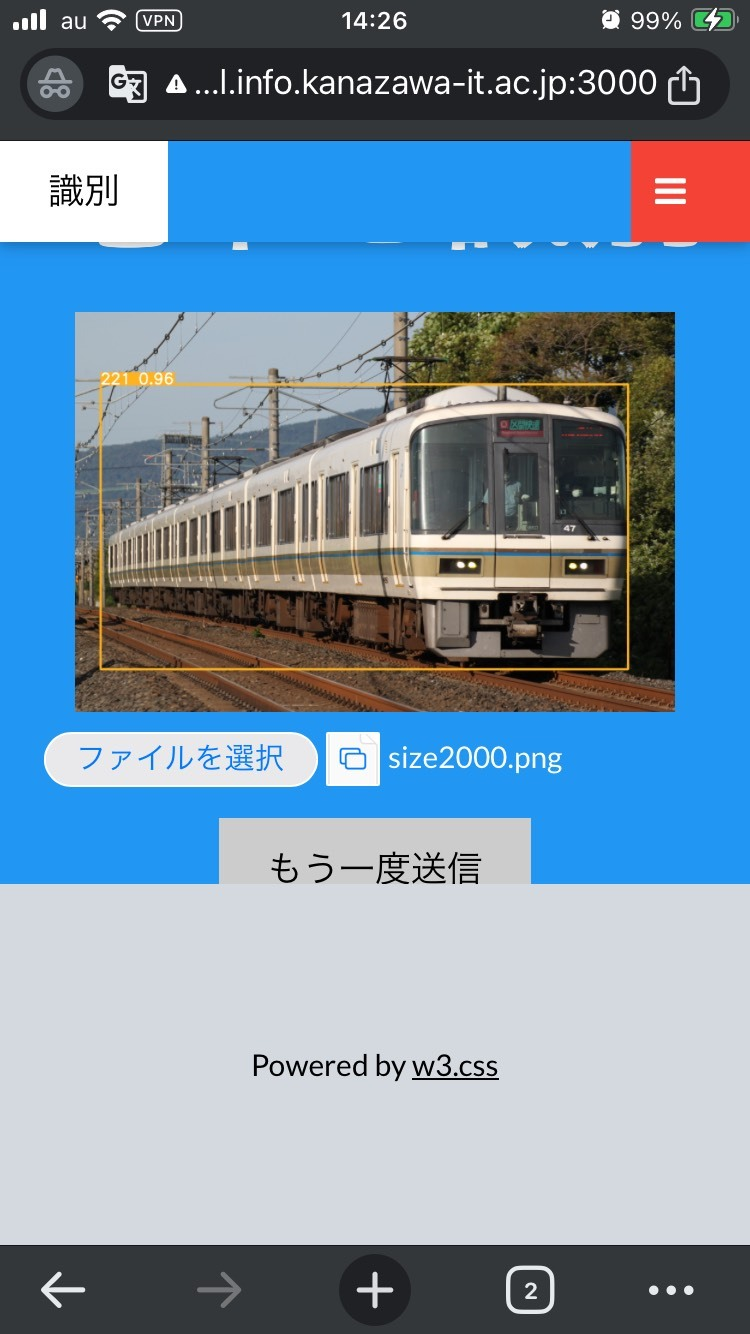
\includegraphics[width=\linewidth]{obj/img_identify.jpg}
			\figcap{画像の識別}{Image Identification}{img_det}
		\end{minipage}
		\begin{minipage}[b]{0.3\textwidth}
			\centering
			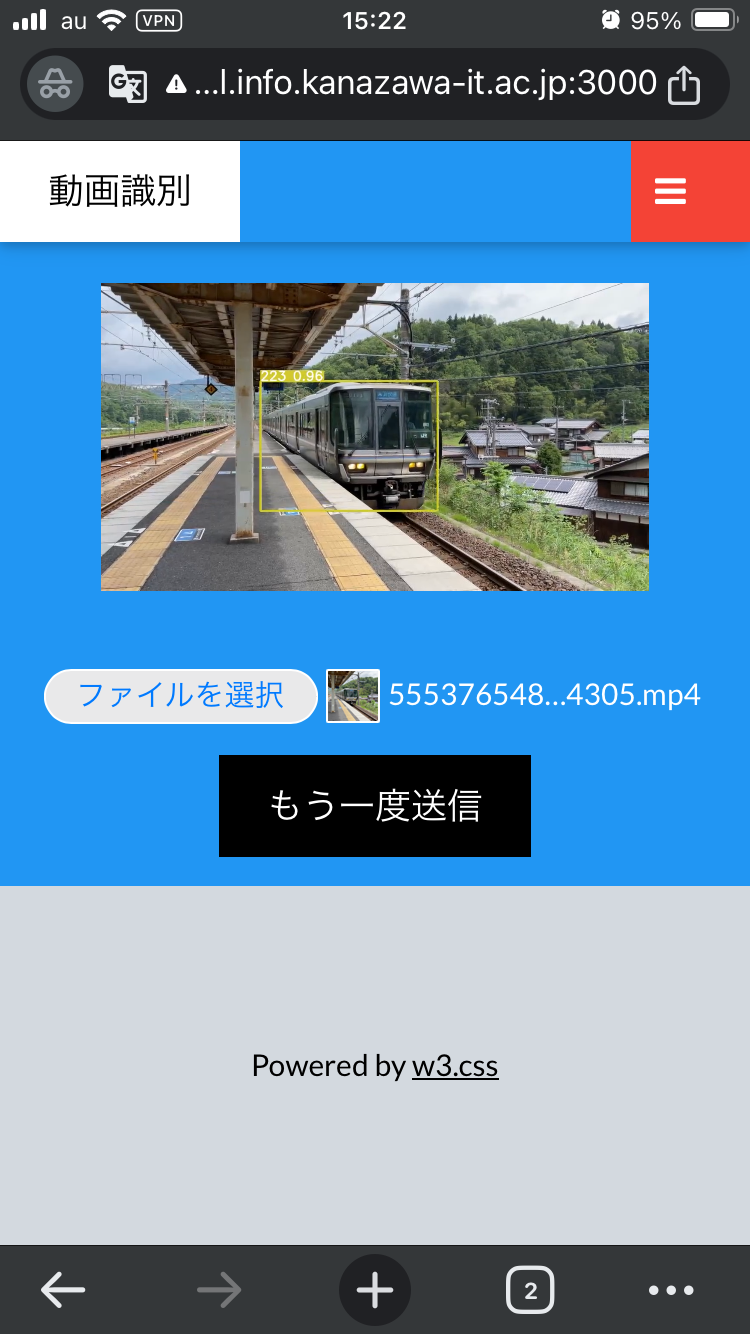
\includegraphics[width=\linewidth]{obj/mov_identify1.jpg}
			\figcap{動画の識別}{Video Identification}{mov_det}
		\end{minipage}
	\end{tabular}
\end{figure}
%https://link-blog.hatenablog.com/entry/2022/10/15/192639を参照

\section{動作確認と現状}
学内ネットワークからWebアプリケーションに接続すると画像の分類,画像の識別,動画の識別の動作を確認できた.
しかしスマホで4G回線に接続し,学内のVPNを用いた際の結果が返される速度と学内ネットワークを用いた際の結果が返される時間に大きな差が出てしまう.
今後,メモリ使用量や,CPU使用量,ネットワーク使用量について調査する.
%ここまで田村

\section{判別モデルの開発の流れ}
電車が写っている画像を集めて,データセットを作成し,学習をするという流れで判別モデルを開発する.

\subsection{データ収集}
YouTubeで特定の電車のみが映っている1〜3種類の動画を保存し,指定した枚数分のランダムなフレームを保存する.保存した画像を識別し電車が映っている画像だけを保存してトレーニングデータとバリデーションデータを収集した.テストデータは様々なウェブサイトから手作業で17種類の各車両の画像を10枚ずつ収集した.
各車両タイプの画像の保存枚数を図\ref{fig:chartdet}に示す.
% TODO: \usepackage{graphicx} required
\subsection{データセットの作成}
本プロジェクトで作成するモデルは識別モデル,分類モデルの二種類である.
%データセットのディレクトリ構造が識別用と分類用で異なるので,それぞれのデータセットを作成した.識別モデルには画像のアノテーション情報も必要なので,アノテーションを行い,識別モデル用のデータセットを作成した.
分類モデルのデータセット内の画像をアノテーションして,識別モデル用のデータセットを作成した.


\subsection{モデルの学習}
%本プロジェクトでは\\
作成したデータセットとYOLOv8~\cite{bk1}を用いてモデルの学習を行い,分類モデルと識別モデルを作成した.
分類モデルでは静止画での判別しかできない.動画から車両タイプを判別するために識別モデルを作成した.

%\subsubsection{学習の実行}
%学習を進めると徐々に性能が上がっていき性能が向上しなくなると学習が途中で中断される.
%学習は中断されるまで続けたため,学習回数はモデルによって差がある.
%識別モデルと分類モデルをどのように使えば結果が出力されるのかを説明する.pythonのコードを貼り付ける?
%田村のパートに記載してもいいかもしれない



\section{作成したモデルの評価と考察}
\subsection{分類モデルの評価}
作成した分類モデルを用いてテストデータセットの分類を行って得られた混同行列を図\ref{fig:classifyresults}に示す.
縦軸は正解の車両タイプを表し,横軸は作成したモデルが予想した車両タイプを表す.

\subsection{識別モデルの評価}
%17種類の車両タイプの画像をそれぞれ10枚ずつ集めテストデータを作成し識別を行った.識別の結果を表\ref{detection}に示す.
%captionを追加するとエラーが発生してしまう
作成した識別モデルを用いてテストデータセットの識別を行って得られた混同行列を図\ref{fig:chartdet}に示す.
識別時には,どの車両タイプにも当てはまらないと識別されることがある.その場合の車両タイプは0として識別モデルの混同行列を作成した.
% TODO: \usepackage{graphicx} required





\subsection{考察}
正解率は電車によって異なることがわかる.287系と683系のように外見が似ている電車だと,誤判別していることが多かった.
287系を図\ref{287},683系を図\ref{683}に示す.
%データセットの画質を落とすと誤判別が増えた.特に誤分類が多かった三種類の電車の画質を上げても結果はあまり変わらなかった.
%限られたストレージでは,データセットの画質を変化させて判別結果を向上させることは難しいと考えられる.SSDの容量に制限がない場合,大量の高画質のデータでデータセットを作成することで判別結果が改善される可能性があると考えられる.
%各車両タイプの画像の枚数に差があったことが判別結果に影響を与えていると考えられる.
データセットの画像の枚数が少ない車両タイプの判別結果が必ず悪くはならなかった.
画像の枚数が判別結果に影響を与えるのではなく,車体の特徴が鮮明に写っている画像の枚数が判別結果に影響を与えると考えられる.
判別精度の向上のために,データセットとして質の悪い画像を大量に集めるのではなく,車体の特徴が鮮明に写っている画像を車両タイプごとに集める必要があったと考えられる.

同じ画像を使って,2種類のデータセットを作成した.分類結果の図と識別結果の図が似ているため,車両タイプを知るためのシステムを作る際には,識別モデルのみを作成することで画像と動画の両方に対応した車両判別システムを作成でき,電車の車両タイプを知ることができるようになると考える.

\section{まとめ}
本プロジェクトでは,機械学習を用いた電車の車両タイプを判別するため,2種類のモデルを作成した.また,電車が写っている画像や動画をサーバ上で,分類,識別を行い判別結果を出力するWebアプリを作成した.

本システムを利用することで電車の知識がない人でも画像または動画に写る一部の車両タイプが何なのかを知ることができる.
4G回線と学内のVPNを利用して判別した場合と,学内ネットワークを利用して判別した場合では,結果が返ってくる時間に大きな差があった.
今後,メモリ使用量やCPU使用量,ネットワーク使用量について調査をする.

\begin{thebibliography}{99}
	%\bibitem{jp2k1} 織田 信長, 明智 光秀, "JPEG2000画像符号化システムにおける係数ビットモデリングと適応算術符号化,"Journal of signal processing(基礎シリーズ), vol.7, no.4, pp.257-266, July 2003.
	%\bibitem{sdkguide}Parrot, "AR.Drone Developer Guide SDK 2.0"
	%\bibitem{bk1} "金沢の暮らし", \url{http://www.kanazawa-it.ac.jp}
	%\bibitem{bk2} 山田 太郎, "金沢の一人暮らし", トンチンカン出版, 2016.

	%\bibitem{bk1}"アノテーションとは - 定義と重要性,必要な準備や注意点を解説",\url{https://www.dir.co.jp/world/entry/solution/annotation}
	
	\bibitem{bk0}"W3.CSS Templates",\url{https://www.w3schools.com/w3css/w3css_templates.asp}
	%\bibitem{bk1}"ファイル:JR West 221 Yamatoji rapid.jpg",\url{https://ja.wikipedia.org/wiki/ファイル:JR_West_221_Yamatoji_rapid.jpg}
	\bibitem{bk1}"Ultralytics YOLOv8 ドキュメント",\url{https://docs.ultralytics.com/ja}
\end{thebibliography}


\begin{figure}
	\centering
	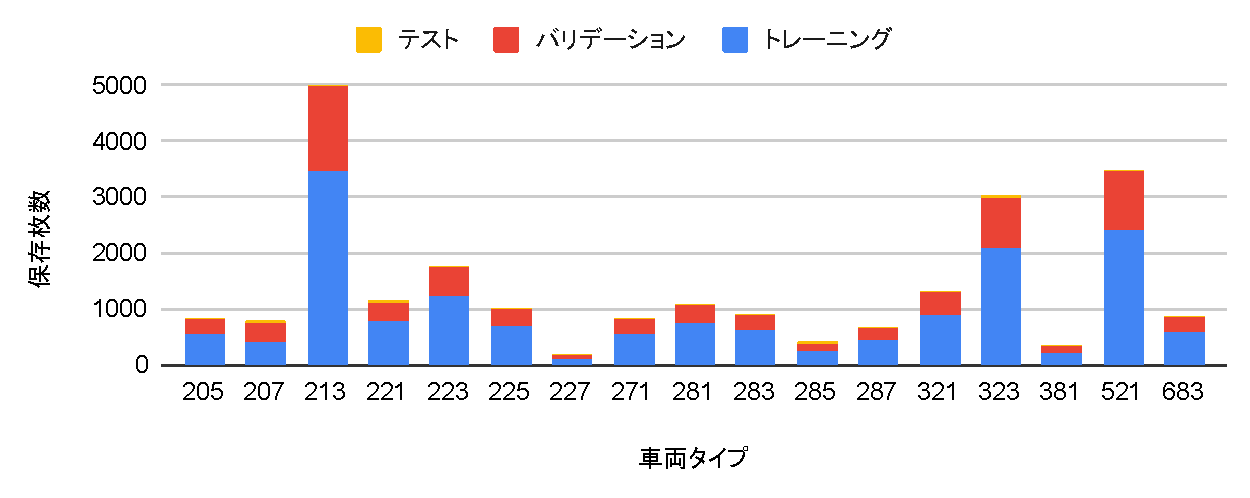
\includegraphics[width=\linewidth]{obj/chart2.pdf}
	\figcap{各車両タイプの保存枚数}{Number of images stored for each type}{fig:chart}
\end{figure}


\begin{figure}
	\centering
	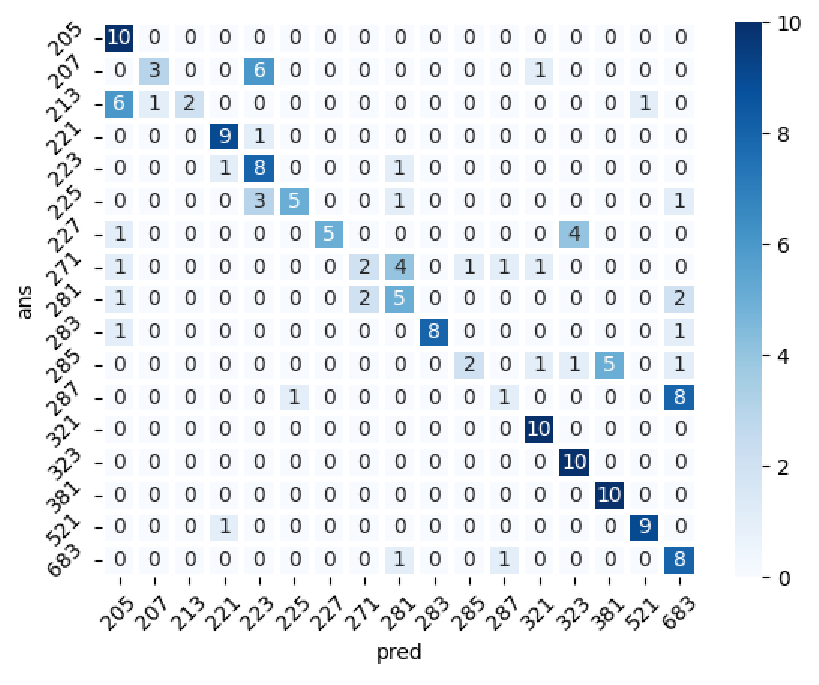
\includegraphics[width=\linewidth]{obj/classify_results.pdf}
	\figcap{分類モデルの混同行列}{Confusion matrix of classification models}{fig:classifyresults}
\end{figure}


\begin{figure}
	\centering
	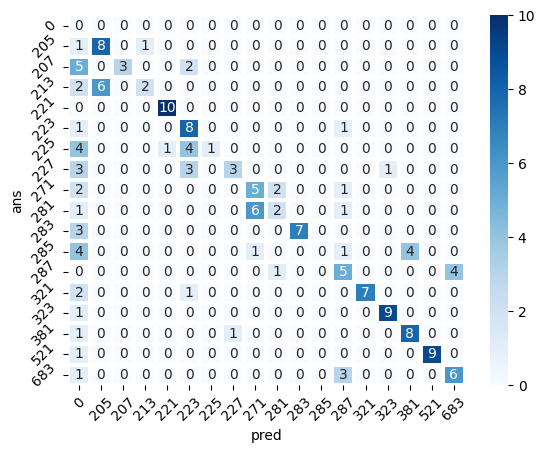
\includegraphics[width=\linewidth]{obj/predicted_results.jpg}
	\figcap{識別モデルの混同行列}{Confusion matrix of identification models}{fig:chartdet}
\end{figure}


\begin{figure}
	\begin{tabular}{cc}
		\begin{minipage}[b]{0.45\textwidth}
			\centering
			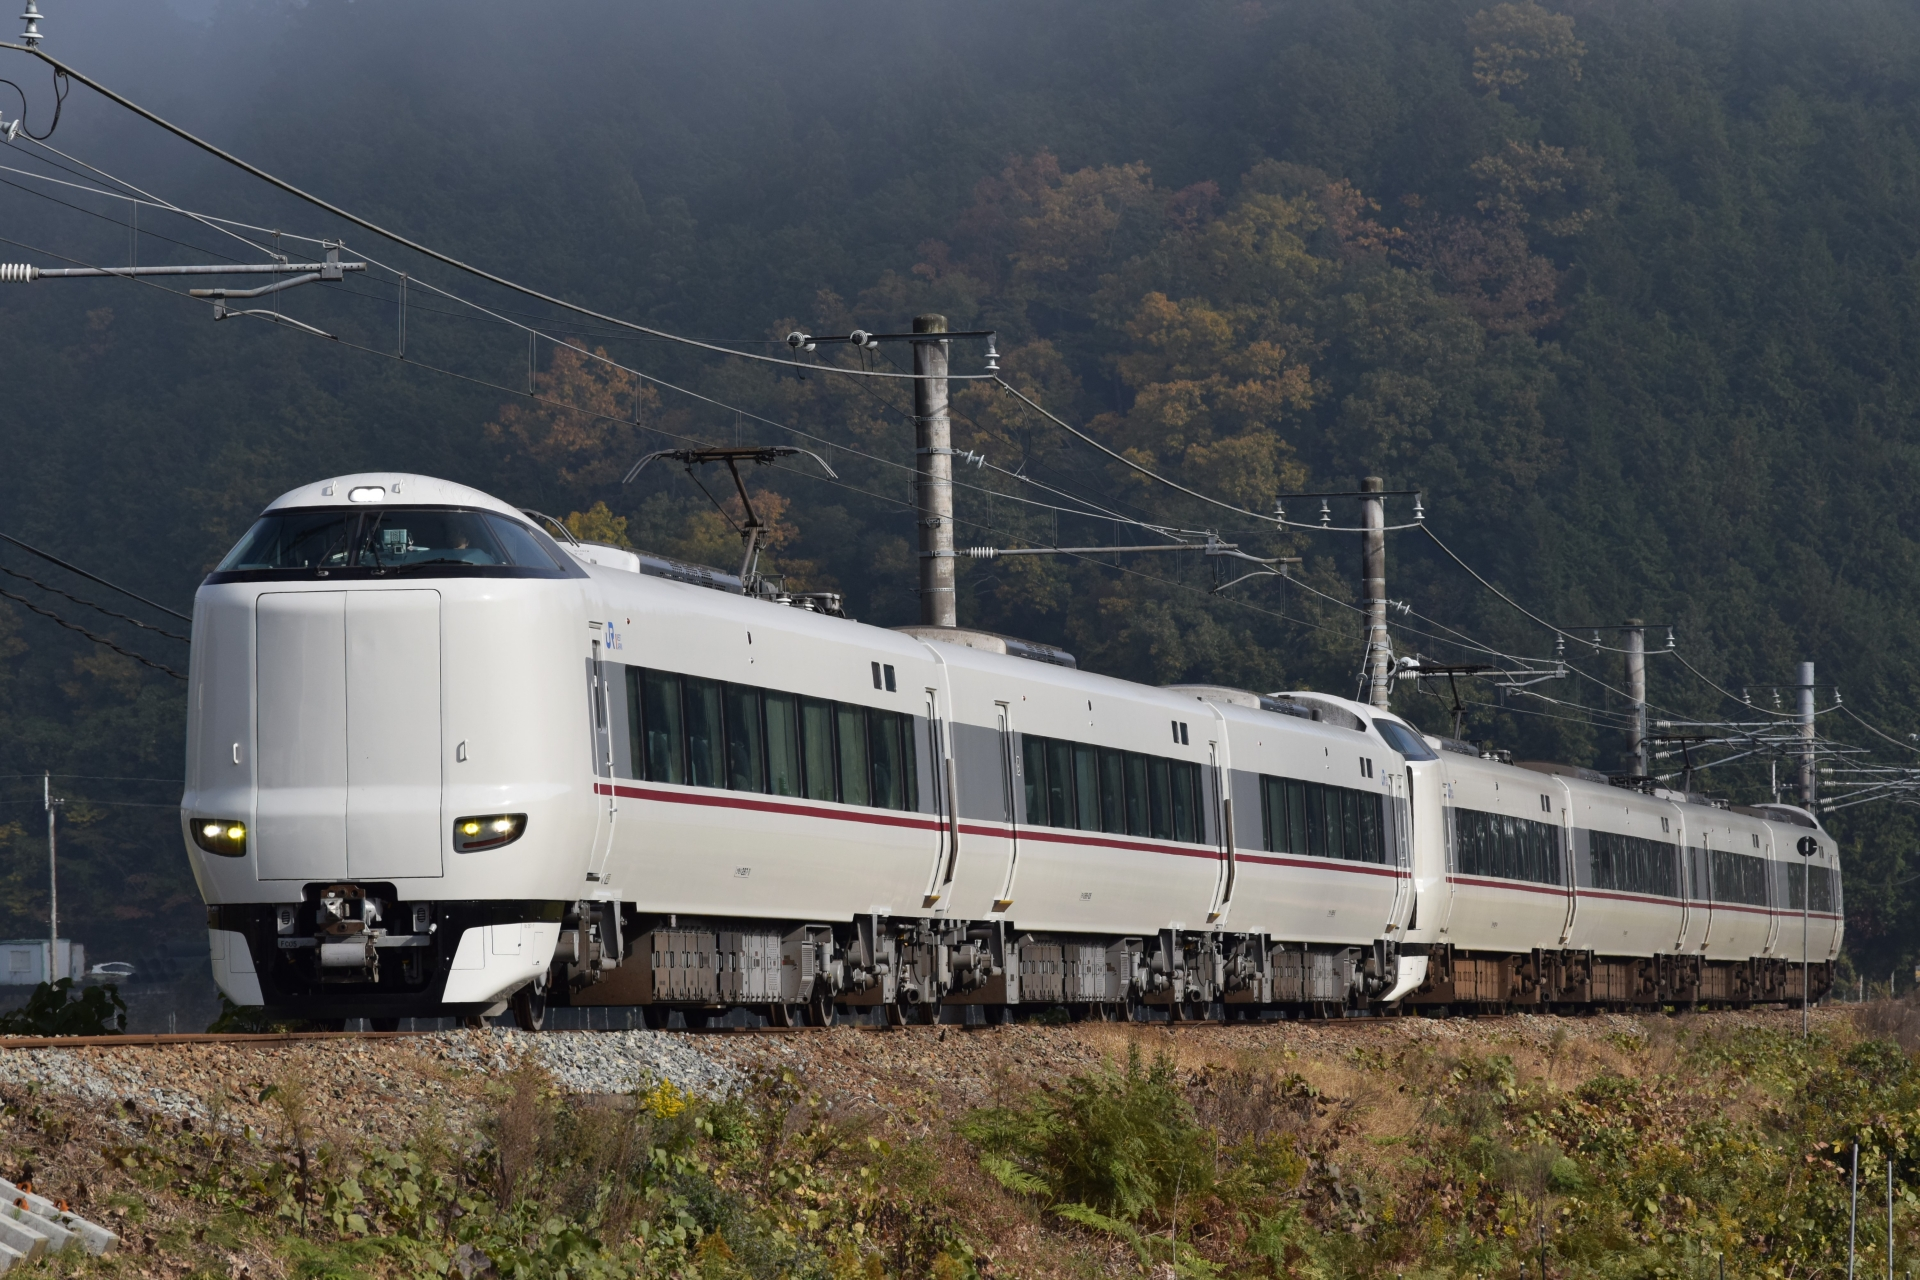
\includegraphics[width=\linewidth]{obj/287.jpg}
			\figcap{287系}{287 series}{287}
		\end{minipage}
		\begin{minipage}[b]{0.45\textwidth}
			\centering
			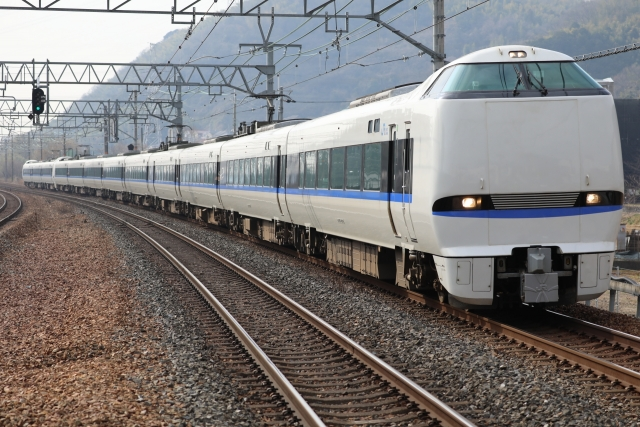
\includegraphics[width=\linewidth]{obj/683.jpg}
			\figcap{683系}{683 series}{683}
		\end{minipage}
	\end{tabular}
\end{figure}




%\noindent\textbf{本プロジェクトに関する業績} % 学部
% \noindent\textbf{本研究に関する業績} % 院生の場合
%\begin{enumerate}[label=\arabic*),leftmargin=2.25\zw]
%\item 鈴木 大志 , 鷹合 大輔 , 中沢 実,"AutoVCを用いたゼロショットリアルタイム声質変換手法の提案",2021-DPS-189(5), 1-6 (2021-12-13) , 2188-8906.
%\end{enumerate}

% 本文ここまで ------------------------------------------------------------------
\end{multicols*} 
\end{document}

